\scanpage{148}
% archive sheet number: 147
\uline{\unsure{Modules|Module} $\ell$-adiques sur} $S$.

Soit $S$ un préschéma, $\ell$ nb premier, \deleted{\unsure{un}} \deleted{\unsure{Ind} \illegible{1}} $\unsure{\mathscr G|\mathcal G}(S)$ la catégorie des schémas en groupes \inserted{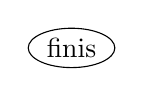
\begin{tikzpicture}[baseline=(n.base)]\node (n) at (0,0) {finis};\draw (0,0) ellipse (.55 and .25);\end{tikzpicture}} étales sur $S$. Un objet de $\operatorname{Ind}(\mathscr G(S))$ est dit ``de type $\mathbb Q_\ell/\mathbb Z_\ell$'' s'il est \uline{strict}, et si ses fibres géométriques sont des \unsure{limites inductives} isomorphes \unsure{à|:} $(\mathbb Q_\ell/\mathbb Z_\ell)^{\unsure{\nu|v}}$ ($\nu$ convenable). Si $S$ est connexe, \deleted{$\xi$ un pt géométrique de $S$, \unsure{alors}} \inserted{$\nu$ est indépendant du} choix du pt géométrique de $S$. Si $\xi$ est un tel pt géométrique, la \deleted{\unsure{anti}} catégorie des \deleted{\unsure{$\mathscr G$}} $G$ ``de type $\mathbb Q_\ell/\mathbb Z_\ell$'' est \deleted{isomorphe} équivalente à la catégorie des \deleted{\unsure{$\xi$}} $\pi_1(S,\xi)$-Modules discrets qui sont isomorphes comme groupes abéliens à $(\mathbb Q_\ell/\mathbb Z_\ell)^\nu$, \deleted{\unsure{donc}} ($\nu$ convenable) i.e. dont le dual au sens de \unsure{Pontrjagin|Pontryagin} [à valeurs dans $\mathbb Q/\mathbb Z$) est \deleted{\unsure{iso}} un module libre de type fini sur $\mathbb Z_\ell^{\deleted{\unsure{\nu|2}}}$.

Par dualité (de Pontrjagin) on obtient les objets de $\operatorname{Pro}\mathscr G(S)$ qui sont ``de type $\mathbb Z_\ell^\nu$''.

Un objet de $\operatorname{Ind}\operatorname{Pro}\mathscr G(S)$ est dit
